Local development of the project was designed to be easy to setup and reproducible in any development machine. For this purpose development virtual machine(dev-vm) is created using infrastructure-as-a-code principle. Tools which are used for reproducible creation of machine were:
\begin{itemize}
    \item Oracle Virtualbox\cite{virtual_box} - hypervisor which is hosting vm, it was chosen because it supports deployment in 3 most popular operating systems: Micrsoft windows, mac os and Linux.
    \item HashiCorp Vagrant\cite{vagrant} - tool which help to build development environment as a code. It allows to specify all details of provisioned vm, as well as configure networking and hardware specifications. All files used for development can be found in dev-vm repository\cite{dev_vm}.
\end{itemize}

Base of the development virtual machine is Ubuntu Linux server so it is not shipped with graphical user interface. It was chosen to resemble production environment, lower vm blueprint and increase speed and performance of the setup. To interact with the machine Secure Shell Protocol (SSH) is used, it can be seen on picture \ref{fig:local_development}.

\begin{figure}[H]
    \centering
    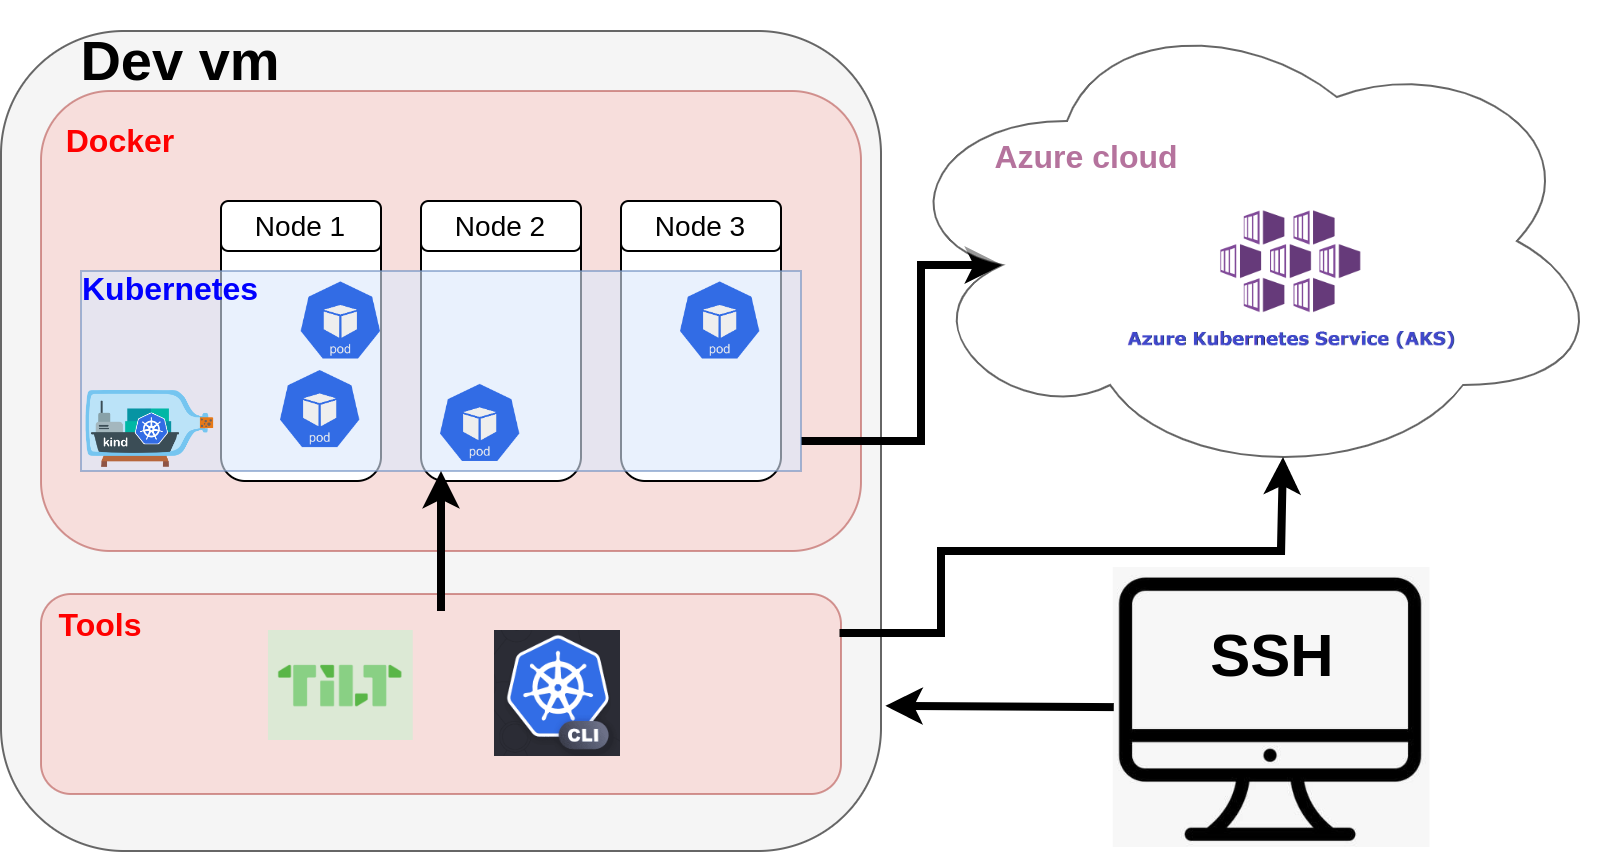
\includegraphics[width=0.8\textwidth]{pictures/development_setup.png}
    \caption{ Local development }
    \label{fig:local_development}
\end{figure}

By default Kubernetes(k8s) cluster is deployed in dev-vm using tool called kind. It allows to create kubernetes nodes as containers and form a kubernetes(k8s) cluster. It can be then accessed with kubernetes client command line tool called kubectl. To speed up development process and allow continuous testing of both software and deployment, tilt is used. This software interact with k8s cluster by building container images and deploying resources as soon as there is any change in the code. It also includes a dashboard \ref{fig:tilt} which visualize resources deployed in a cluster as well as aggregates the logs and show them in approachable matter.


\begin{figure}[H]
    \centering
    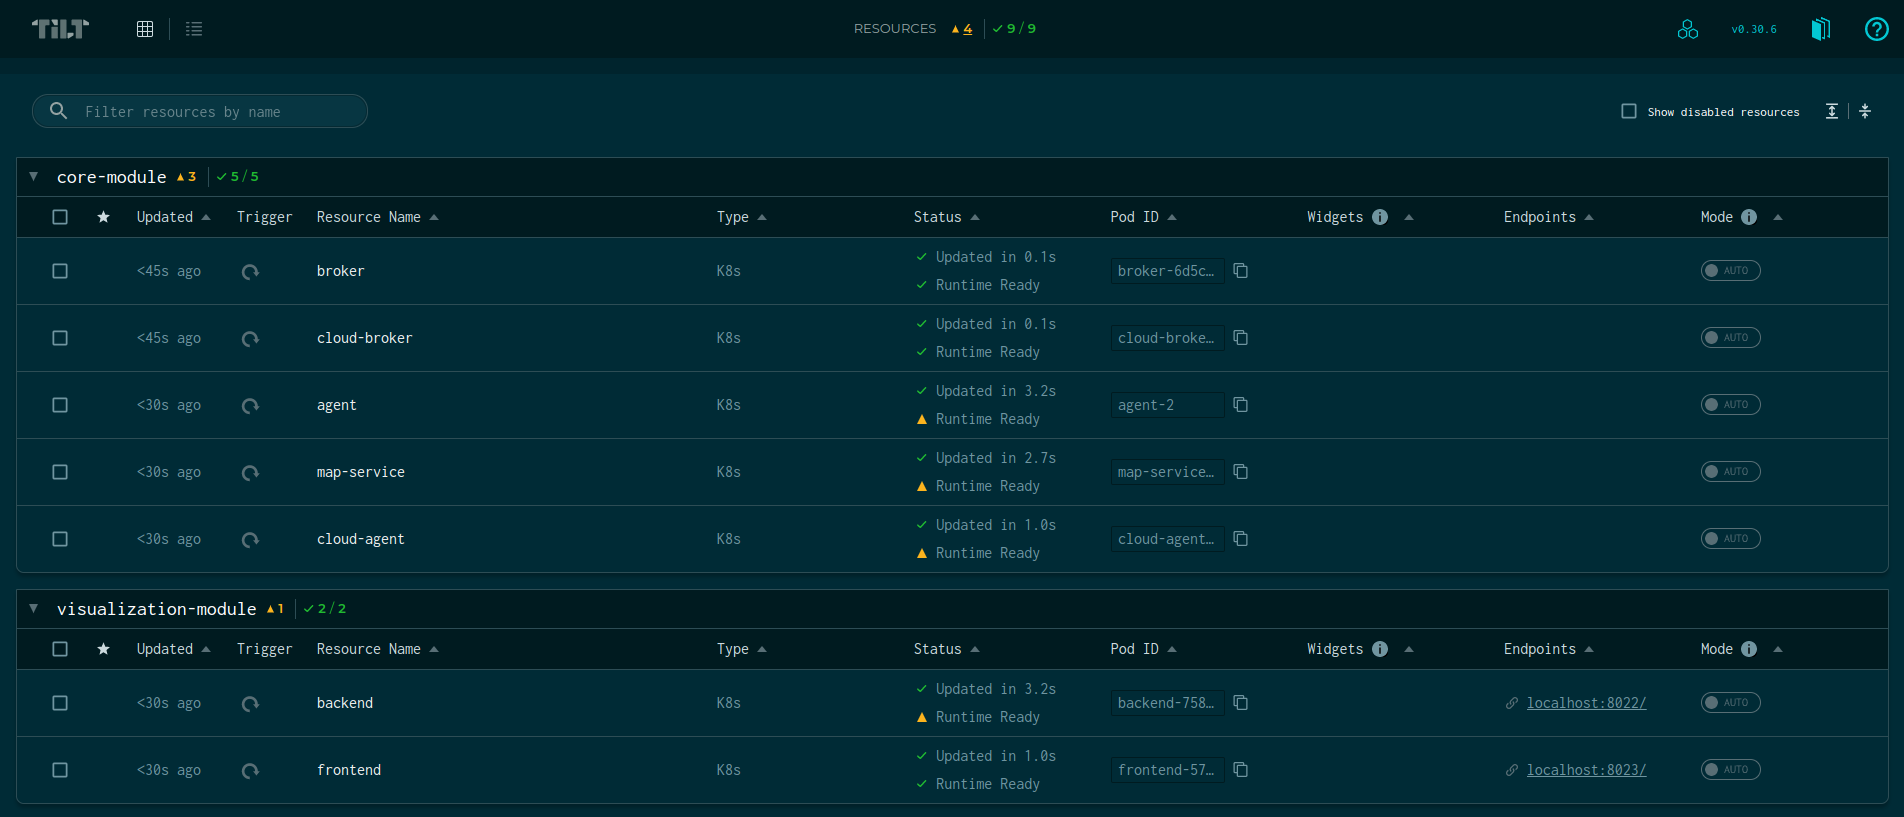
\includegraphics[width=\textwidth]{pictures/tilt.png}
    \caption{ Tilt dashboard}
    \label{fig:tilt}
\end{figure}

Integration with a azure cloud is made with azure command lines tools along with PAT token. After initial creation of kubernetes cluster in the cloud, interaction are limited to only kubernetes cluster and therefore only kubeconfig file is needed.

To make it easier to interact with ll resources used in the project, set of make rules was set up and includes:
\begin{itemize}
    \item make dev - run dev cluster and tilt
	\item make clean - stop local cluster and tilt
	\item make cloud-login - login to azure and setup kubectl
	\item make cloud-up - start kubernetes cluster in azure
	\item make cloud-down - stop kubernetes cluster in azure
	\item make cloud-deploy - deploy to kubernetes cluster in azure
	\item make cloud-build - build and push docker images
	\item make local-observability - deploy observability stack to local cluster
	\item make pdf - generate this document in form of pdf
\end{itemize}